\documentclass{standalone}
\usepackage[mode=buildnew]{standalone}
\usepackage{tikz}
\usepackage{amssymb}
\usetikzlibrary{positioning, shapes, arrows, patterns}

\begin{document}
\begin{tikzpicture}
    \node[circle, draw, thick, minimum size=5cm] (s) {$s$};
    \node[above=0.1cm of s] (Po) {$\mathcal{B}(s, \epsilon)$};
    \node[circle, thick, minimum size=5cm, below right of=s] (o11) {$o_1$};
    \node[circle, thick, minimum size=5cm, above right of=s] (o21) {$o_2$};
\end{tikzpicture}
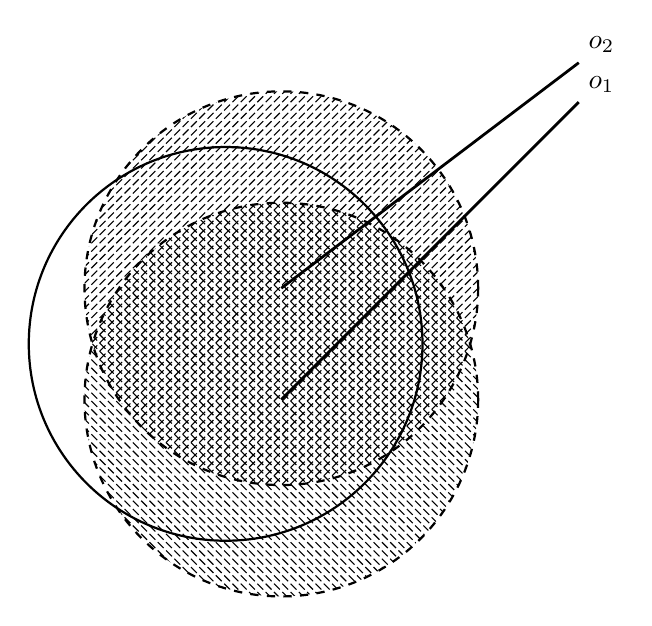
\begin{tikzpicture}
    \node[circle, draw, thick, minimum size=5cm] (s) {};
    \node[circle, dashed, draw, thick, minimum size=5cm, pattern=north west lines, below right of=s] (o11) {};
    \node[above right=2cm and 2cm of o11] (o12) {$o_1$};
    \node[circle, dashed, draw, thick, minimum size=5cm, pattern=north east lines, above right of=s] (o21) {};
    \node[above right=2.5cm and 2cm of o11] (o22) {$o_2$};
    
    
    \draw[-, line width=1pt] (o11.center) -- (o12.south west) {};
    \draw[-, line width=1pt] (o21.center) -- (o22.south west) {};
\end{tikzpicture}
\end{document}